\documentclass[]{emulateapj}
\PassOptionsToPackage{hyphens}{url}\usepackage{hyperref}
\usepackage{natbib}
\usepackage{amssymb}
\usepackage{color}
\usepackage{amsmath,mathtools}
\usepackage{epsfig}
\usepackage[FIGTOPCAP]{subfigure}
\usepackage{afterpage}
\usepackage{enumerate}
\usepackage{multirow}
\usepackage{verbatim}
\usepackage{relsize}
\usepackage{tikz}
\usetikzlibrary{shapes.geometric, arrows}
\usepackage{morefloats}
\usepackage{wasysym}

\newcommand{\noop}[1]{}
\newcommand{\note}[1]{{\color{red} #1}}
\newcommand{\cn}{\note{(cite)}}
\newcommand{\unit}[1]{\ensuremath{\, \mathrm{#1}}}
\newcommand{\mearth}{\unit{M_\oplus}}
\newcommand{\rearth}{\unit{R_\oplus}}
\newcommand{\msun}{\unit{M_\odot}}
\newcommand{\lsun}{\unit{L_\odot}}
\newcommand{\mstar}{\unit{M_\star}}
\newcommand{\rj}{\ensuremath{R_\mathrm{J}}}
\newcommand{\avg}[1]{\langle #1 \rangle}
\newcommand{\bavg}[1]{\bigg\langle #1 \bigg\rangle}
\newcommand{\tab}[1]{\hspace{.2\textwidth}\rlap{#1}}
\DeclareMathOperator*{\argmin}{arg\,min}

\shorttitle{Proxima Centauri b Water Loss}
\shortauthors{Rodrigo Luger}

\begin{document}

\title{Proxima Centauri b Water Loss}
\author{Rodrigo Luger}


\section{Intro}
\label{sec:intro}

We perform a suite of Markov Chain Monte Carlo (MCMC) runs to obtain constraints on the
present-day water content of Proxima Centauri b using the Python code package \texttt{emcee}
\citep{ForemanMackey13}. MCMC allows one to sample from multi-dimensional probability 
distributions that are difficult or impossible to obtain directly, which is the case for
the ensemble of parameters that control the evolution of the planet surface water content
in \texttt{VPLANET}. In this section, we develop a framework for inferring the probability 
distributions of these parameters conditioned on empirical data and our understanding
of the physical processes at play.

The input parameters to our model make up the state vector $\mathbf{x}$:
%
\begin{align}
\label{eq:mcmcx}
\mathbf{x} = \{f_\mathrm{sat}, t_\mathrm{sat}, \beta_\mathrm{xuv}, M_\star, t_\star, a, m\},
\end{align}
%
corresponding, respectively, to the stellar mass, the XUV saturation fraction, the XUV saturation timescale,
the XUV power law exponent, the stellar age, the semi-major axis of the planet, and the
mass of the planet. Given a value of $\mathbf{x}$, \texttt{VPLANET} computes the evolution of the system from
time $t = 0$ to $t = t_\star$, yielding the output vector $\mathbf{y}$:
%
\begin{align}
\label{eq:mcmcy}
\mathbf{y}(\mathbf{x}) = \{L_\star, L_\mathrm{xuv}, t_\mathrm{RG}, m_\mathrm{H}, m_\mathrm{H_2O}, m_\mathrm{O_2}\},
\end{align}
%
corresponding, respectively, to the stellar luminosity, the stellar XUV luminosity, the duration of the 
runaway greenhouse phase, the mass of the
planet's hydrogen envelope, the mass of water remaining on its surface, and the mass of oxygen retained
in either the atmosphere or the surface/mantle, all of which are evaluated at $t = t_\star$ (i.e., the present day). 
Additional parameters that control the evolution of the 
planet (initial water content, XUV absorption efficiency, etc.) are held fixed in individual runs; see below.

Our goal in this section is to derive posterior distributions for $\mathbf{y}$ (and in particular for $m_\mathrm{H_2O}$) 
given prior information on both 
$\mathbf{x}$ and $\mathbf{y}$. Some parameters---such as the present-day stellar luminosity---are well-constrained,
while others are less well-known and will thus be informed primarily by our choice of prior. This is the case for
the XUV saturation fraction, saturation timescale, and power law exponent, which have been studied in detail 
for solar-like stars \citep{Ribas05} but are poorly constrained for M dwarfs. \note{More info on them here...}
We therefore use flat-log priors for the saturation fraction and timescale, enforcing
$-5 \leq \log(f_\mathrm{sat}) \leq -2$ and $-0.3 \leq \log(t_\mathrm{sat} / \mathrm{Gyr}) \leq 1$. We use
a Gaussian prior for the XUV power law exponent, with a mean of 1.23, the value derived by \citep{Ribas05} for
solar-like stars: $\beta_\mathrm{xuv} \sim \mathcal{N}(-1.23, 0.1)$. We choose an ad hoc standard deviation
$\sigma = 0.1$ \note{because...}

We also use a flat prior for the stellar mass ($0.1 \leq M_\star / \mathrm{M}_\oplus \leq 0.15$).
Although stronger constraints on the stellar mass exist \cn, these are derived indirectly from mass-luminosity relations; we thus
enforce a prior on the present-day luminosity to constrain the value of $M_\star$ via our stellar evolution model (see below).
We enforce a Gaussian prior on the stellar age $t_\star \sim \mathcal{N}(4.8, 1.4^2)$ Gyr based on the constraints discussed
in \S\cn. 

Our prior on the semi-major axis $a$ is a combination of a Gaussian prior on the orbital period, 
$P \sim \mathcal{N}(11.186, 0.002^2)$ days \citep{AngladaEscude16}, and the stellar mass prior. 
Finally, our prior on the planet mass $m$ combines the empirical minimum mass distribution,
$m\sin i \sim \mathcal{N}(1.27, 0.18^2)$ M$_\oplus$ \citep{AngladaEscude16}, and the a priori inclination distribution
for randomly aligned orbits, 
$\sin i \sim \mathcal{U}(0, 1)$, where $\mathcal{U}$ is a uniform distribution \citep[e.g.,][]{Luger17}.

We further condition our model on measured values of the stellar luminosity $L_\star$ and 
stellar XUV luminosity $L_\mathrm{xuv}$. We take
$L_\star \sim \mathcal{N}(1.65, 0.15) \times 10^{-3}$ L$_\odot$ \citep{Demory09} and 
$\log L_\mathrm{xuv} \sim \mathcal{N}(-6.36, 0.3^2)$. We base the latter on \cite{Ribas16}, who compiled a comprehensive
list of measurements of the emission of Proxima Centauri in the wavelength range 0.6--118 nm. Summing the fluxes over
this range and neglecting the contribution of flares, we obtain an XUV flux at Proxima Centauri b 
$F_\mathrm{xuv} \approx 252\ \mathrm{erg\ cm^{-2}\ s^{-1}}$, corresponding to $\log L_\mathrm{xuv} = -6.36$ for $a = 0.0485$ AU. Given the
lack of uncertainties for many of the values compiled in \cite{Ribas16} and the fact that some of those estimates
are model extrapolations, it is difficult to establish a reliable error estimate for this value. We make the 
ad hoc but conservative choice $\sigma = 0.3$ dex, noting that the three measurements that inform the X-ray luminosity 
of the star in \cite{Ribas16} (which dominates its XUV emission) have a spread corresponding to $\sigma = 0.2$ dex. 
However, more rigorous constraints on the XUV emission of Proxima Cen with reliable uncertainties are direly needed
to obtain more reliable estimates of water loss from Proxima Cen b.

Given these constraints, we wish to find the posterior distribution of each of the parameters in Equations~(\ref{eq:mcmcx}) 
and~(\ref{eq:mcmcy}). We thus define our likelihood function $\mathcal{L}$ for a given state vector $\mathbf{x}$ as
%
\begin{align}
\ln \mathcal{L}(\mathbf{x}) = &- \frac{1}{2}\left[\frac{(L_\mathrm{\star}(\mathbf{x}) - L_\mathrm{\star})^2}{\sigma_{L_\star}^2}
                               - \frac{(L_\mathrm{xuv}(\mathbf{x}) - L_\mathrm{xuv})^2}{\sigma_{L_\mathrm{xuv}}^2}\right]
                                 \nonumber\\
                              &+ \ln \mathrm{Prior}(\mathbf{x}) + C,
\end{align}
%
where $L_\mathrm{\star}(\mathbf{x})$ and $L_\mathrm{xuv}(\mathbf{x})$ are, respectively, the model predictions for the present-day 
stellar luminosity and stellar XUV luminosity given the state vector $\mathbf{x}$, $L_\mathrm{\star}$ and $L_\mathrm{xuv}$ are
their respective observed values, and $\sigma_{L_\star}^2$ and $\sigma_{L_\mathrm{xuv}}^2$ are the uncertainties on those observations. The
$\ln \mathrm{Prior}(\mathbf{x})$ term is the prior probability and $C$ is an arbitrary normalization constant. Expressed in this form,
the observed values of $L_\mathrm{\star}$ and $L_\mathrm{xuv}$ are our ``data,'' while the constraints on the other parameters
are ``priors,'' though the distinction is purely semantic.

\begin{figure}[hbt]
  \begin{center}
      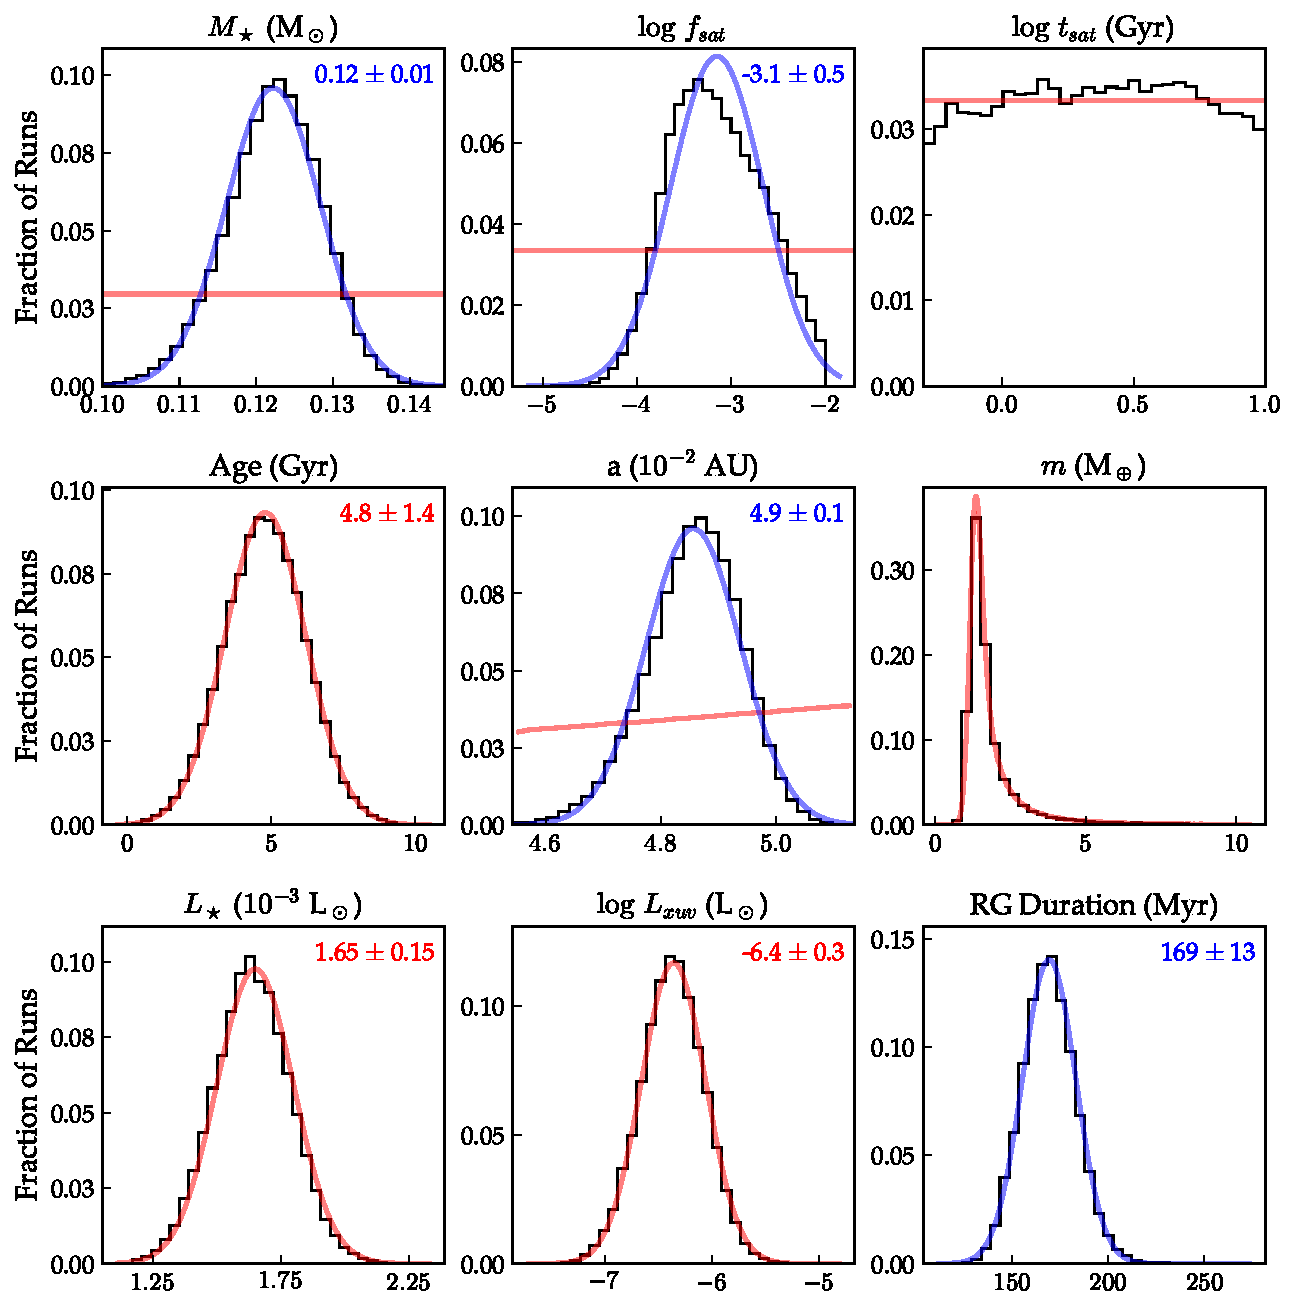
\includegraphics[width=0.45\textwidth]{figures/star_posteriors.pdf}
       \caption{Posterior distributions for the various stellar parameters used in the model. The first eight
                parameters are model inputs, with their corresponding priors shown in red. The combination of
                these priors and the physical models in \texttt{VPLANET} constrain the stellar and planetary
                parameters shown in this section. Blue curves show Gaussian fits to the posterior distributions,
                with the mean and standard deviation indicated at the top right.
                The last panel shows the duration of the runaway greenhouse
                phase for Proxima Centauri b, one of the model outputs, which we find to be 169 $\pm$ 13 Myr.}
     \label{fig:star_posteriors}
  \end{center}
\end{figure}

Given this likelihood function, we use MCMC to obtain the posterior probability distributions for each of the parameters
of interest. We draw each of the $\mathbf{x}$ from their respective prior distributions and run 40 parallel chains of 5,000 
steps each, discarding the first 500 steps as burn-in. The posterior distributions for the stellar mass, saturation fraction,
saturation timescale, age, semi-major axis, planet mass, present-day stellar luminosity, present-day stellar XUV luminosity, and 
duration of the runaway greenhouse are shown in Figure~\ref{fig:star_posteriors} as the black histograms. The red curves 
indicate our priors/data, and the purple curve is a Gaussian fit to the runaway greenhouse duration posterior,
yielding $t_\mathrm{RG} = 169 \pm 13$ Myr.

By construction, the planet mass, stellar age, present-day stellar luminosity, and present-day stellar XUV luminosity posteriors reflect
their prior distributions. As mentioned above, the stellar mass posterior is entirely informed by the luminosity posterior via the
\cite{YonseiYale13} stellar evolution tracks. The stellar mass in turn constrains the semi-major axis (via the prior on the period and
Kepler's laws). The XUV saturation fraction 

\begin{figure}[hbt]
  \begin{center}
      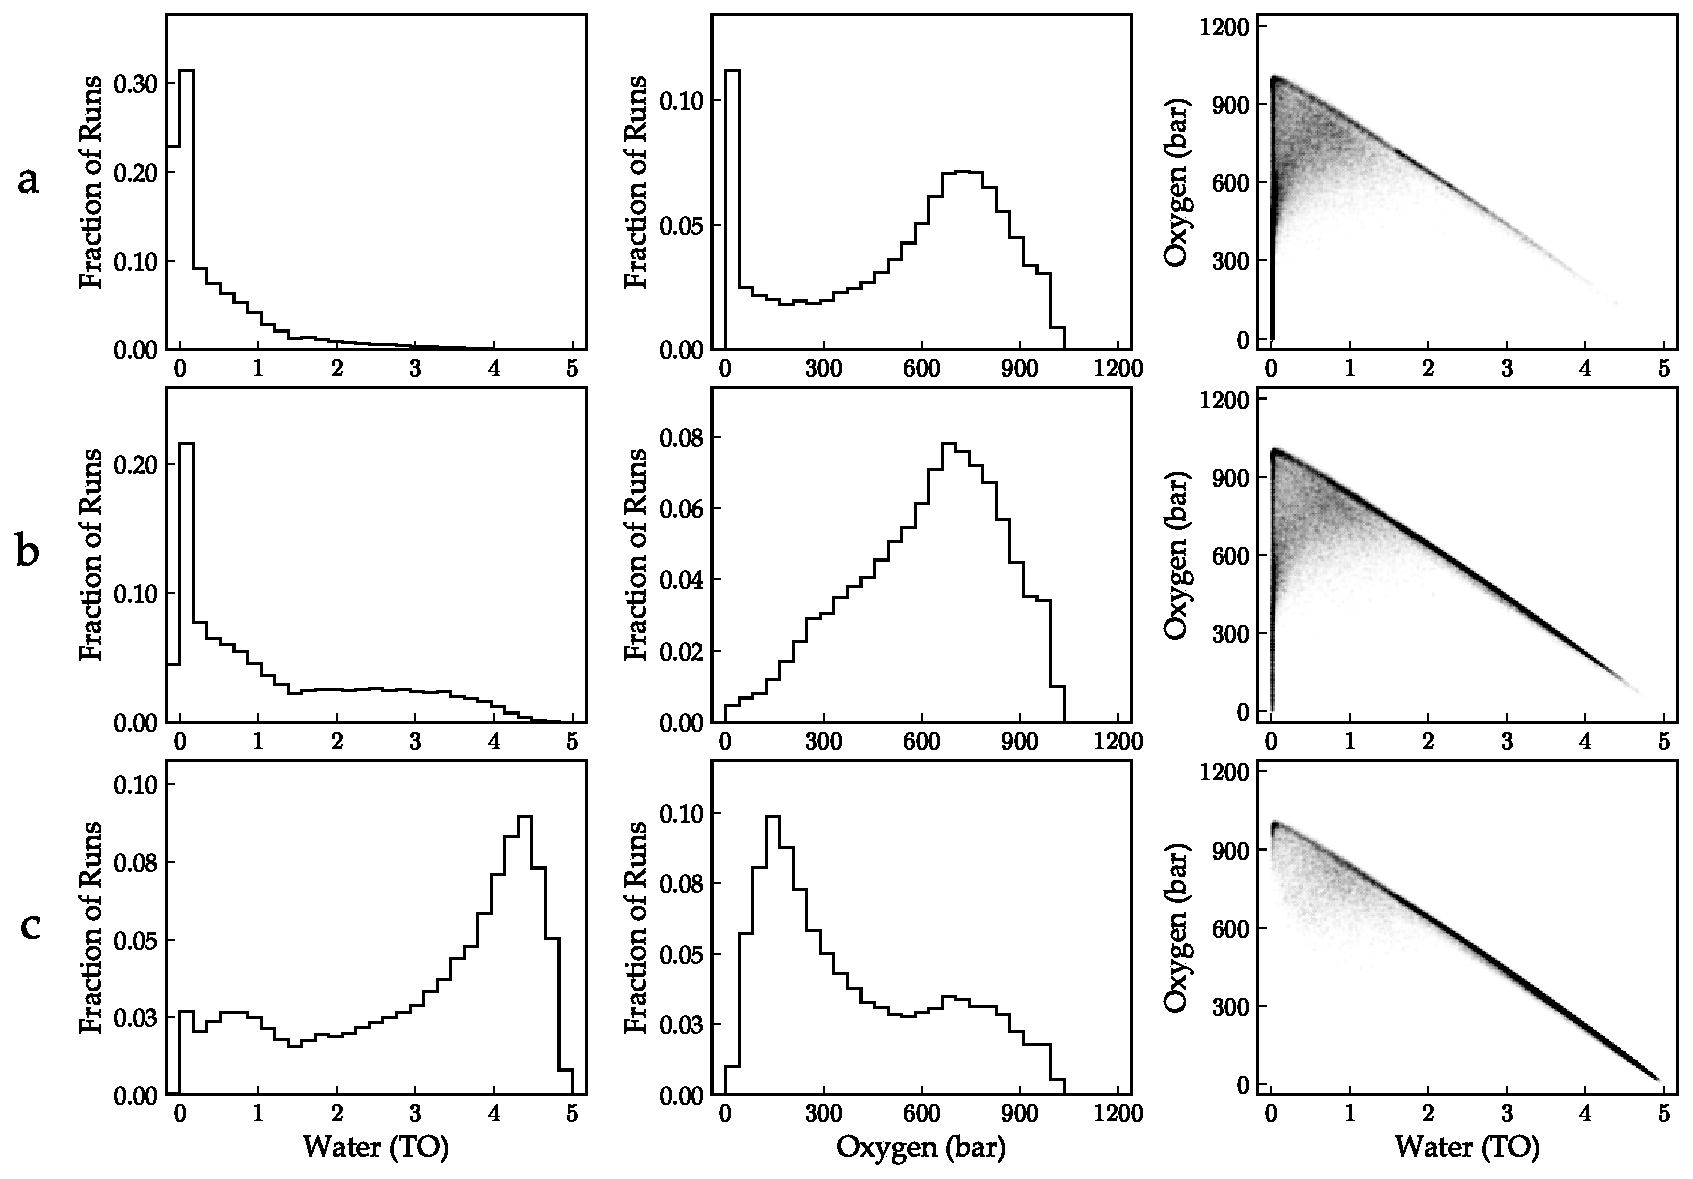
\includegraphics[width=0.45\textwidth]{figures/planet_epsilon.pdf}
       \caption{Planet posteriors (epsilon).}
     \label{fig:planet_epsilon}
  \end{center}
\end{figure}

\begin{figure}[hbt]
  \begin{center}
      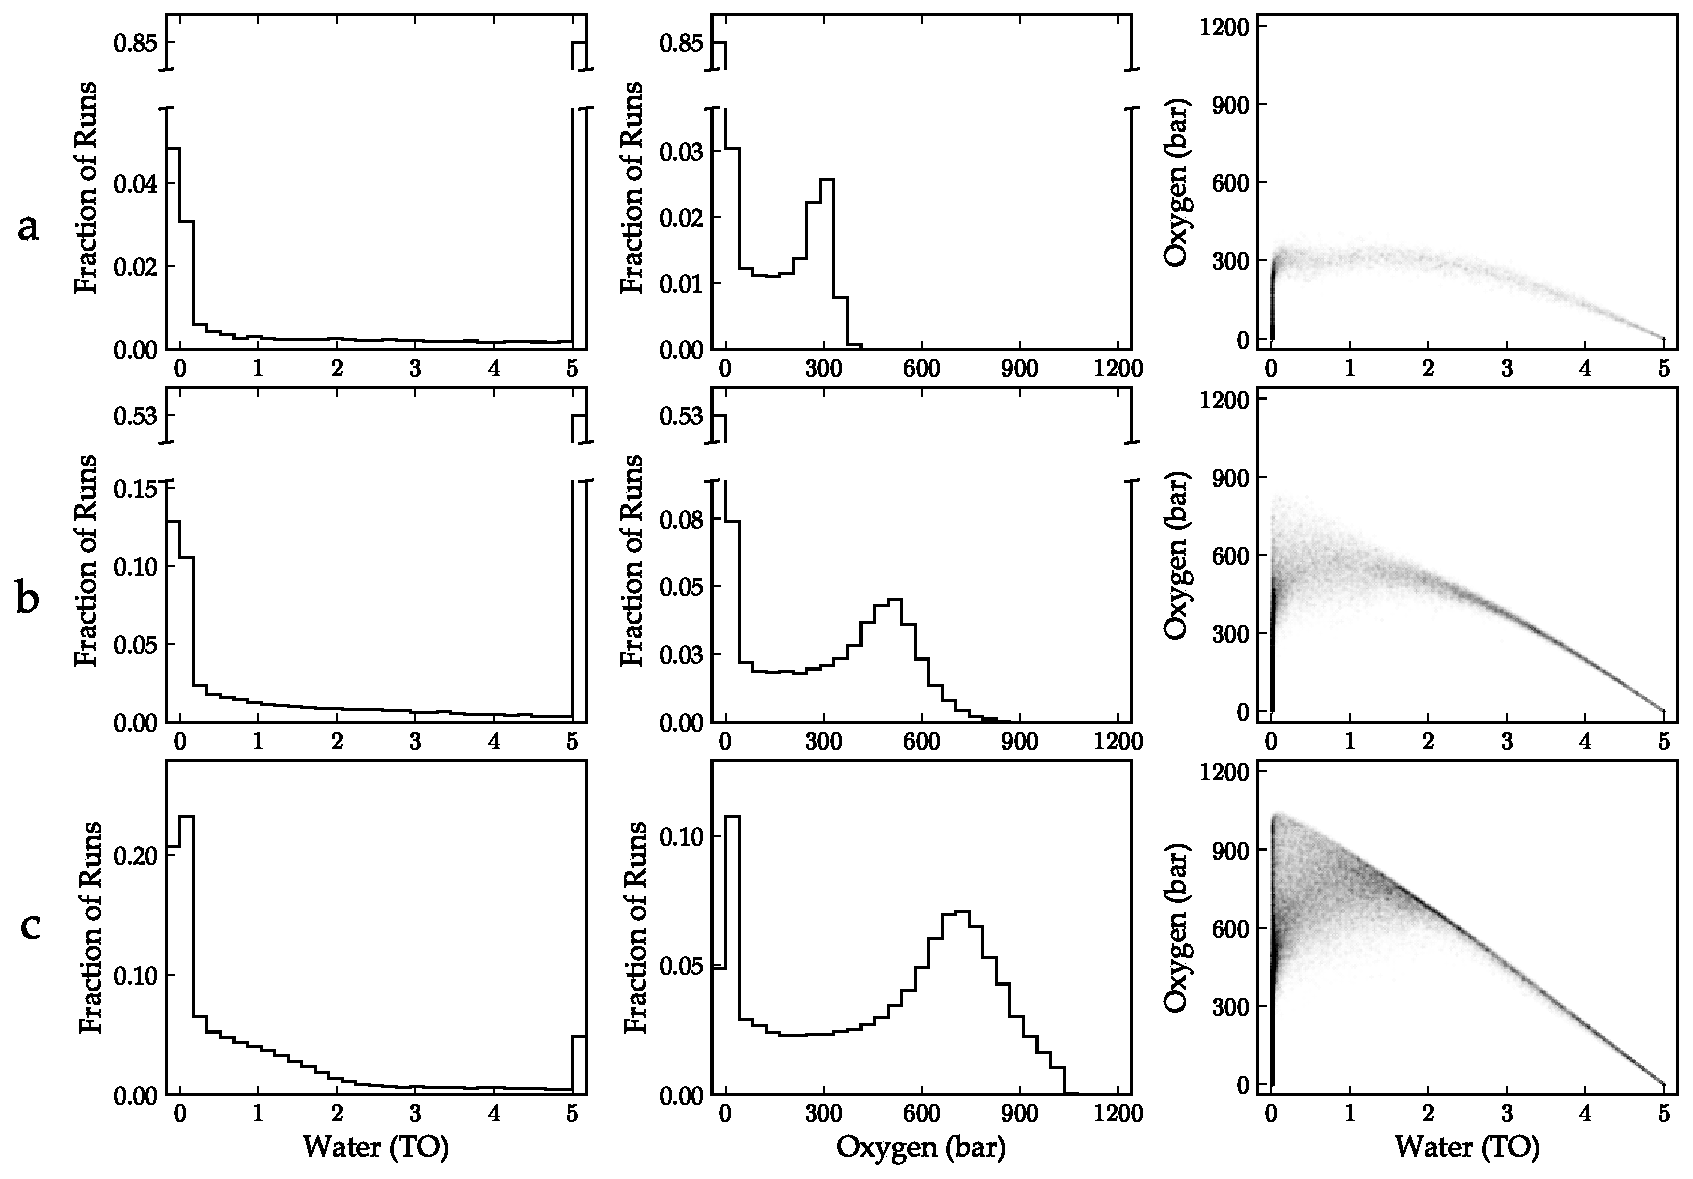
\includegraphics[width=0.45\textwidth]{figures/planet_hydrogen.pdf}
       \caption{Planet posteriors (hydrogen).}
     \label{fig:planet_hydrogen}
  \end{center}
\end{figure}

\begin{figure}[hbt]
  \begin{center}
      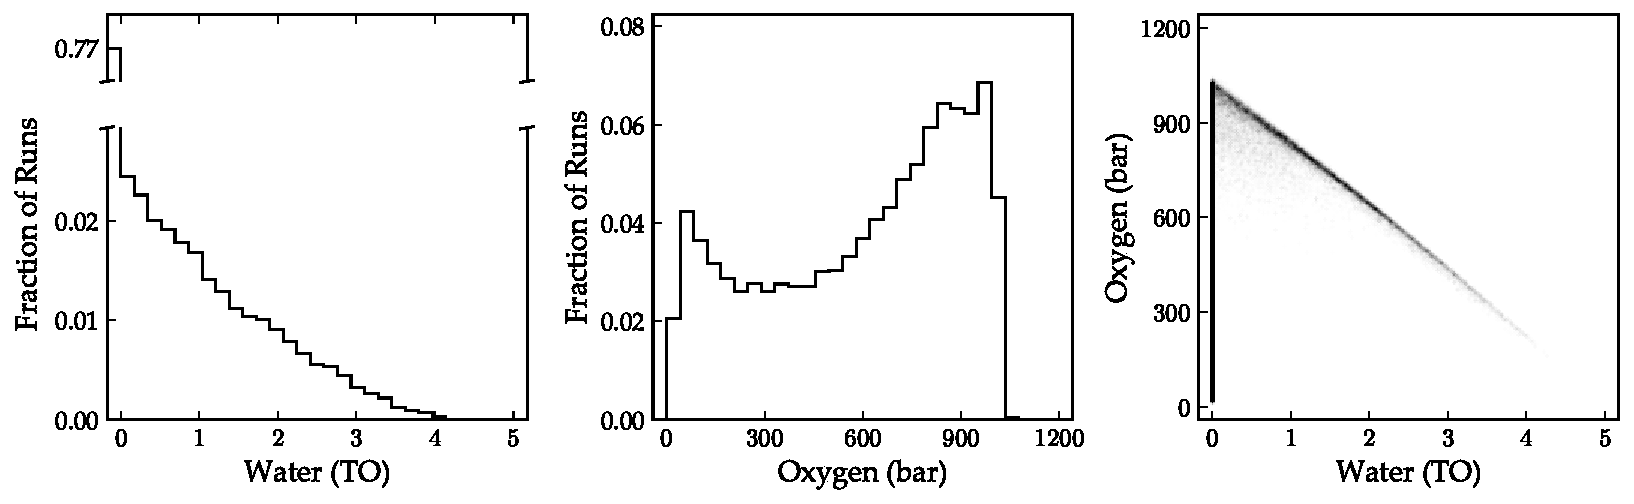
\includegraphics[width=0.45\textwidth]{figures/planet_magma.pdf}
       \caption{Planet posteriors (magma).}
     \label{fig:planet_hydrogen}
  \end{center}
\end{figure}

\begin{figure}[hbt]
  \begin{center}
      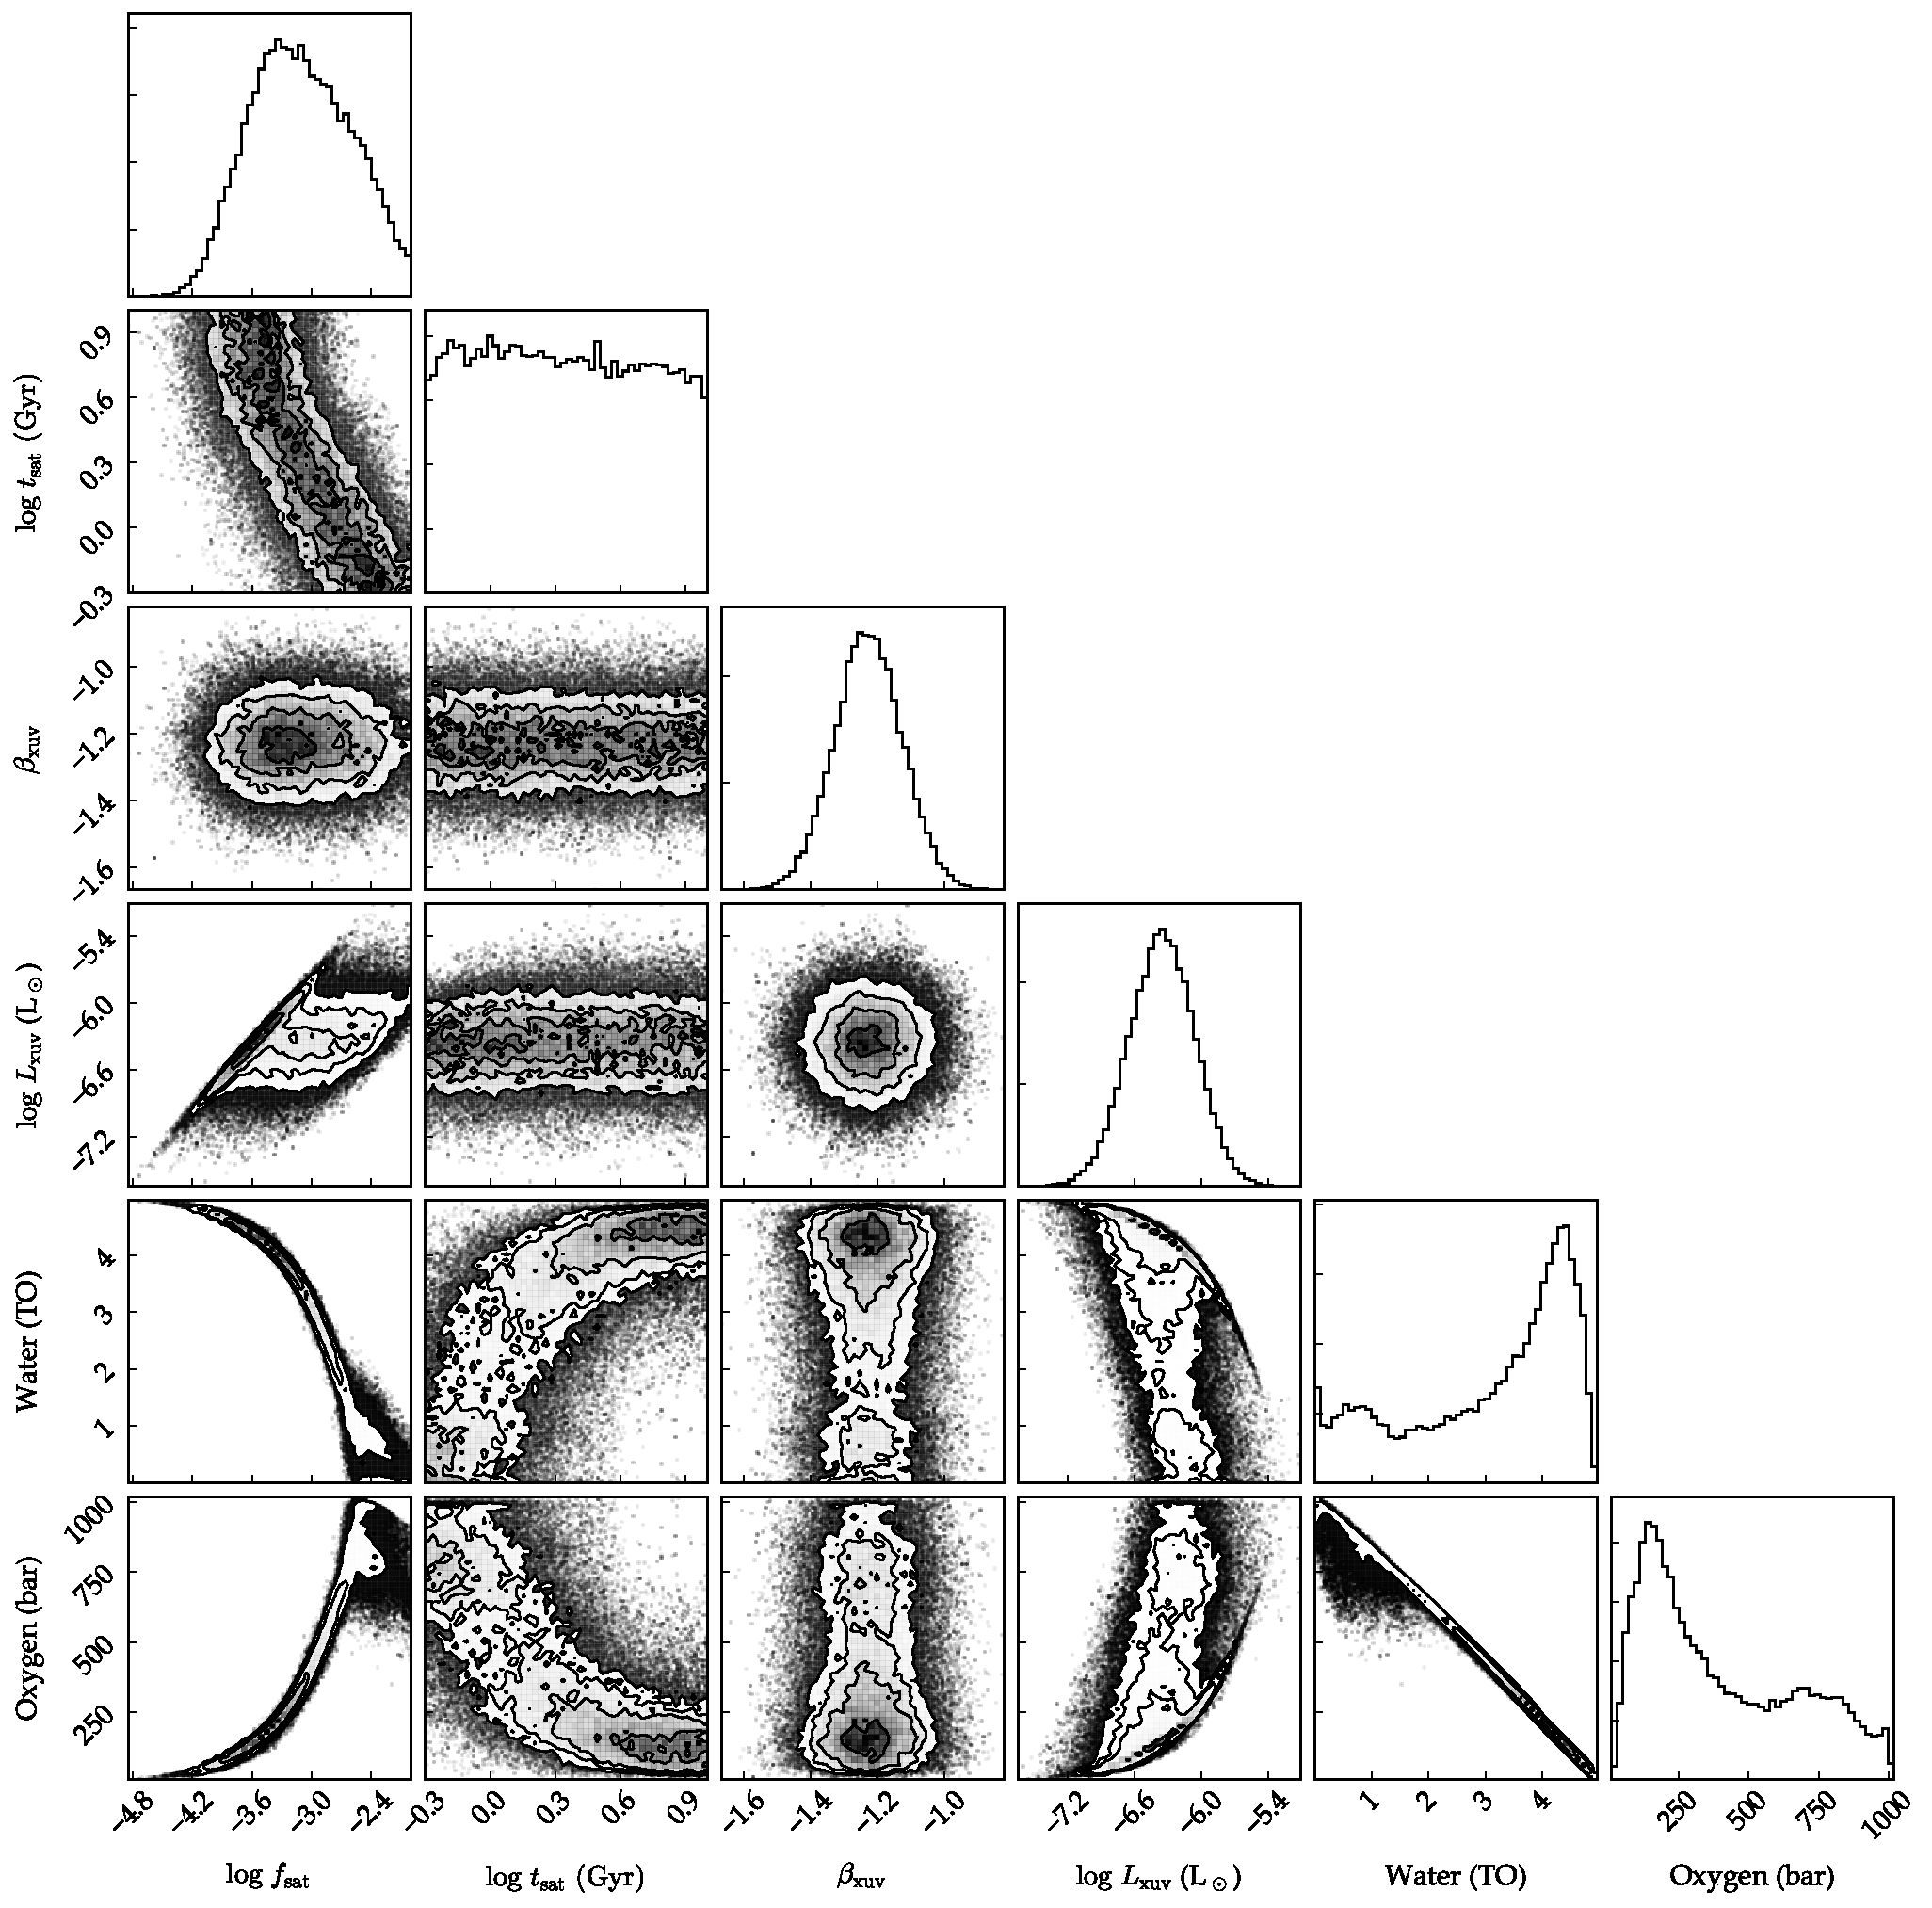
\includegraphics[width=0.45\textwidth]{figures/corner.pdf}
       \caption{Correlations. Beta isn't correlated with water because it's too late to matter.}
     \label{fig:corner}
  \end{center}
\end{figure}

\clearpage
\bibliographystyle{apj}
\bibliography{uncert}

\end{document}